\PassOptionsToPackage{unicode=true}{hyperref} % options for packages loaded elsewhere
\PassOptionsToPackage{hyphens}{url}
%
\documentclass[10pt,]{article}
\usepackage{lmodern}
\usepackage{amssymb,amsmath}
\usepackage{ifxetex,ifluatex}
\usepackage{fixltx2e} % provides \textsubscript
\ifnum 0\ifxetex 1\fi\ifluatex 1\fi=0 % if pdftex
  \usepackage[T1]{fontenc}
  \usepackage[utf8]{inputenc}
  \usepackage{textcomp} % provides euro and other symbols
\else % if luatex or xelatex
  \usepackage{unicode-math}
  \defaultfontfeatures{Ligatures=TeX,Scale=MatchLowercase}
\fi
% use upquote if available, for straight quotes in verbatim environments
\IfFileExists{upquote.sty}{\usepackage{upquote}}{}
% use microtype if available
\IfFileExists{microtype.sty}{%
\usepackage[]{microtype}
\UseMicrotypeSet[protrusion]{basicmath} % disable protrusion for tt fonts
}{}
\IfFileExists{parskip.sty}{%
\usepackage{parskip}
}{% else
\setlength{\parindent}{0pt}
\setlength{\parskip}{6pt plus 2pt minus 1pt}
}
\usepackage{hyperref}
\hypersetup{
            pdftitle={Bridging a gap between mathematics and data in teaching data science and statistics with the R package caracas for computer algebra},
            pdfauthor={Mikkel Meyer Andersen and Søren Højsgaard},
            pdfborder={0 0 0},
            breaklinks=true}
\urlstyle{same}  % don't use monospace font for urls
\usepackage[margin=1in]{geometry}
\usepackage{color}
\usepackage{fancyvrb}
\newcommand{\VerbBar}{|}
\newcommand{\VERB}{\Verb[commandchars=\\\{\}]}
\DefineVerbatimEnvironment{Highlighting}{Verbatim}{commandchars=\\\{\}}
% Add ',fontsize=\small' for more characters per line
\usepackage{framed}
\definecolor{shadecolor}{RGB}{248,248,248}
\newenvironment{Shaded}{\begin{snugshade}}{\end{snugshade}}
\newcommand{\AlertTok}[1]{\textcolor[rgb]{0.94,0.16,0.16}{#1}}
\newcommand{\AnnotationTok}[1]{\textcolor[rgb]{0.56,0.35,0.01}{\textbf{\textit{#1}}}}
\newcommand{\AttributeTok}[1]{\textcolor[rgb]{0.77,0.63,0.00}{#1}}
\newcommand{\BaseNTok}[1]{\textcolor[rgb]{0.00,0.00,0.81}{#1}}
\newcommand{\BuiltInTok}[1]{#1}
\newcommand{\CharTok}[1]{\textcolor[rgb]{0.31,0.60,0.02}{#1}}
\newcommand{\CommentTok}[1]{\textcolor[rgb]{0.56,0.35,0.01}{\textit{#1}}}
\newcommand{\CommentVarTok}[1]{\textcolor[rgb]{0.56,0.35,0.01}{\textbf{\textit{#1}}}}
\newcommand{\ConstantTok}[1]{\textcolor[rgb]{0.00,0.00,0.00}{#1}}
\newcommand{\ControlFlowTok}[1]{\textcolor[rgb]{0.13,0.29,0.53}{\textbf{#1}}}
\newcommand{\DataTypeTok}[1]{\textcolor[rgb]{0.13,0.29,0.53}{#1}}
\newcommand{\DecValTok}[1]{\textcolor[rgb]{0.00,0.00,0.81}{#1}}
\newcommand{\DocumentationTok}[1]{\textcolor[rgb]{0.56,0.35,0.01}{\textbf{\textit{#1}}}}
\newcommand{\ErrorTok}[1]{\textcolor[rgb]{0.64,0.00,0.00}{\textbf{#1}}}
\newcommand{\ExtensionTok}[1]{#1}
\newcommand{\FloatTok}[1]{\textcolor[rgb]{0.00,0.00,0.81}{#1}}
\newcommand{\FunctionTok}[1]{\textcolor[rgb]{0.00,0.00,0.00}{#1}}
\newcommand{\ImportTok}[1]{#1}
\newcommand{\InformationTok}[1]{\textcolor[rgb]{0.56,0.35,0.01}{\textbf{\textit{#1}}}}
\newcommand{\KeywordTok}[1]{\textcolor[rgb]{0.13,0.29,0.53}{\textbf{#1}}}
\newcommand{\NormalTok}[1]{#1}
\newcommand{\OperatorTok}[1]{\textcolor[rgb]{0.81,0.36,0.00}{\textbf{#1}}}
\newcommand{\OtherTok}[1]{\textcolor[rgb]{0.56,0.35,0.01}{#1}}
\newcommand{\PreprocessorTok}[1]{\textcolor[rgb]{0.56,0.35,0.01}{\textit{#1}}}
\newcommand{\RegionMarkerTok}[1]{#1}
\newcommand{\SpecialCharTok}[1]{\textcolor[rgb]{0.00,0.00,0.00}{#1}}
\newcommand{\SpecialStringTok}[1]{\textcolor[rgb]{0.31,0.60,0.02}{#1}}
\newcommand{\StringTok}[1]{\textcolor[rgb]{0.31,0.60,0.02}{#1}}
\newcommand{\VariableTok}[1]{\textcolor[rgb]{0.00,0.00,0.00}{#1}}
\newcommand{\VerbatimStringTok}[1]{\textcolor[rgb]{0.31,0.60,0.02}{#1}}
\newcommand{\WarningTok}[1]{\textcolor[rgb]{0.56,0.35,0.01}{\textbf{\textit{#1}}}}
\usepackage{graphicx,grffile}
\makeatletter
\def\maxwidth{\ifdim\Gin@nat@width>\linewidth\linewidth\else\Gin@nat@width\fi}
\def\maxheight{\ifdim\Gin@nat@height>\textheight\textheight\else\Gin@nat@height\fi}
\makeatother
% Scale images if necessary, so that they will not overflow the page
% margins by default, and it is still possible to overwrite the defaults
% using explicit options in \includegraphics[width, height, ...]{}
\setkeys{Gin}{width=\maxwidth,height=\maxheight,keepaspectratio}
\setlength{\emergencystretch}{3em}  % prevent overfull lines
\providecommand{\tightlist}{%
  \setlength{\itemsep}{0pt}\setlength{\parskip}{0pt}}
\setcounter{secnumdepth}{5}
% Redefines (sub)paragraphs to behave more like sections
\ifx\paragraph\undefined\else
\let\oldparagraph\paragraph
\renewcommand{\paragraph}[1]{\oldparagraph{#1}\mbox{}}
\fi
\ifx\subparagraph\undefined\else
\let\oldsubparagraph\subparagraph
\renewcommand{\subparagraph}[1]{\oldsubparagraph{#1}\mbox{}}
\fi

% set default figure placement to htbp
\makeatletter
\def\fps@figure{htbp}
\makeatother

\usepackage{amsmath}
\usepackage{natbib}
\usepackage{fancyvrb}
\DeclareMathOperator{\logit}{logit}
\DeclareMathOperator{\bin}{bin}
\usepackage[]{natbib}
\bibliographystyle{plainnat}

\title{Bridging a gap between mathematics and data in teaching data science and
statistics with the \texttt{R} package \texttt{caracas} for computer
algebra}
\author{Mikkel Meyer Andersen and Søren Højsgaard}
\date{}

\begin{document}
\maketitle

\def\EE{\mathbf{E}}
\def\var{\mathbf{Var}}
\def\cov{\mathbf{Cov}}
\def\trace{\mathbf{tr}}
\def\det{\mathbf{det}}
\def\diag{\mathbf{diag}}
\def\proglang#1{\texttt{#1}}
\def\pkg#1{\texttt{#1}}

\def\sympy{\texttt{SymPy}}
\def\python{\texttt{Python}}
\def\caracas{\texttt{caracas}}
\def\r{\texttt{R}}

\def\bb{{b}}

\def\inv{^{-1}}
\def\transp{^\top}
\def\cip{\perp\!\!\perp}

\newcommand{\matrxr}[1]
{\left(
    \begin{array}{rrrrrrrrrrrrrrrrrrrrrrrrrrrrrrrrrrrrr}
      #1 \\
    \end{array}
  \right)}

\newcommand{\matrxc}[1]
{\left(
    \begin{array}{cccccccccccccccccccccccccccccccccccc}
      #1 \\
    \end{array}
  \right)}

\makeatletter
\renewcommand*\env@matrix[1][c]{\hskip -\arraycolsep
  \let\@ifnextchar\new@ifnextchar
  \array{*\c@MaxMatrixCols #1}}
\makeatother

\parindent0pt

\hypertarget{introduction}{%
\section{Introduction}\label{introduction}}

\label{sec:introduction}

The capability of \texttt{R} \citep{R} to handle symbolic mathematics is
enhanced by two add-on packages: The \texttt{caracas} package
\citep{caracas:21} and the \texttt{Ryacas} package \citep{ryacas}. In
this paper we will illustrate the use of the \texttt{caracas} package in
connection with teaching mathematics and statistics, where symbolic
mathematics is helpful, strongly aided by the packages' ability to enter
in a reproducible framework (provided by, e.g.~\texttt{Rmarkdown}
\citep{rmarkdown, RMarkdownDefinitiveGuide, RMarkdownCookbook}). Focus
is on 1) treating statistical models symbolically, 2) on bridging the
gap between symbolic mathematics and numerical computations and 3) on
preparing teaching material. The \texttt{caracas} package is available
from CRAN \citep{R}. The open-source development version of
\texttt{caracas} is available at \url{https://github.com/r-cas/caracas}.

Neither \texttt{caracas} nor \texttt{Ryacas} are as powerful as some of
the larger commercial computer algebra systems (CAS). The virtue of
\texttt{caracas} and \texttt{Ryacas} lie elsewhere: (1) Mathematical
tools like equation solving, summation, limits, symbolic linear algebra,
outputting in tex format etc.~are directly available from within
\texttt{R}. (2) The packages enable working with the same language and
in the same environment as the user does for statistical analyses. (3)
Symbolic mathematics can easily be combined with data which is helpful
in e.g.~numerical optimization. (4) The packages are open-source and
therefore support e.g.~education - also for people with limited
economical means and thus contributing to United Nations sustainable
development goals, cfr. \citep{UN17}.

The paper is organized as follows:\footnote{FINISH LATER} Sec.
\ref{sec:mathintro} introduces the \texttt{caracas} package and its
syntax, including how \texttt{caracas} can be used in connection with
preparing texts, e.g.~teaching material. More details are provided in
the appendix (Sec. \ref{sec:primer}). Several vignettes illustrating
\texttt{caracas} are provided and they are also available online, see
\url{https://r-cas.github.io/caracas/}. Sec. \ref{sec:statistics} is the
main section of the paper and here we present a sample of statistical
models where we believe that a symbolic treatment is a valuable
supplement to a numerical in connection with teaching. Sec.
\ref{sec:topicsstudents} contains suggestions about hand-on activities
for students. Lastly, Sec. \ref{sec:discussion} contains a discussion of
the paper.

\hypertarget{sec:mathintro}{%
\section{Mathematics and documents containing
mathematics}\label{sec:mathintro}}

We start by introducing the \texttt{caracas} syntax on familiar topics
within calculus and linear algebra.

\hypertarget{calculus}{%
\subsection{Calculus}\label{calculus}}

First we define a \texttt{caracas} symbol \texttt{x} (see Sec.
\ref{sec:primer}) and subsequently \texttt{p} to be a polynomial in
\texttt{x} (\texttt{p} becomes a symbol because \texttt{x} is)

\begin{Shaded}
\begin{Highlighting}[]
\NormalTok{R}\OperatorTok{>}\StringTok{ }\KeywordTok{library}\NormalTok{(caracas)}
\NormalTok{R}\OperatorTok{>}\StringTok{ }\KeywordTok{def_sym}\NormalTok{(x) }\CommentTok{## Declares 'x' as a symbol}
\NormalTok{R}\OperatorTok{>}\StringTok{ }\NormalTok{p <-}\StringTok{ }\DecValTok{1} \OperatorTok{-}\StringTok{ }\NormalTok{x}\OperatorTok{^}\DecValTok{2} \OperatorTok{+}\StringTok{ }\NormalTok{x}\OperatorTok{^}\DecValTok{3} \OperatorTok{+}\StringTok{ }\NormalTok{x}\OperatorTok{^}\DecValTok{4}\OperatorTok{/}\DecValTok{4} \OperatorTok{-}\StringTok{ }\DecValTok{3} \OperatorTok{*}\StringTok{ }\NormalTok{x}\OperatorTok{^}\DecValTok{5} \OperatorTok{/}\StringTok{ }\DecValTok{5} \OperatorTok{+}\StringTok{ }\NormalTok{x}\OperatorTok{^}\DecValTok{6} \OperatorTok{/}\StringTok{ }\DecValTok{6}
\NormalTok{R}\OperatorTok{>}\StringTok{ }\NormalTok{p}
\end{Highlighting}
\end{Shaded}

\begin{verbatim}
## c:  6      5    4              
##    x    3*x    x     3    2    
##    -- - ---- + -- + x  - x  + 1
##    6     5     4
\end{verbatim}

The gradient of \texttt{p} is

\begin{Shaded}
\begin{Highlighting}[]
\NormalTok{R}\OperatorTok{>}\StringTok{ }\NormalTok{grad <-}\StringTok{ }\KeywordTok{der}\NormalTok{(p, x) }\CommentTok{## der is shorthand for derivative}
\NormalTok{R}\OperatorTok{>}\StringTok{ }\NormalTok{grad}
\end{Highlighting}
\end{Shaded}

\begin{verbatim}
## c:  5      4    3      2      
##    x  - 3*x  + x  + 3*x  - 2*x
\end{verbatim}

Stationary points of \(p\) can be found by finding roots of the
gradient. In this simple case we can factor the gradient

\begin{Shaded}
\begin{Highlighting}[]
\NormalTok{R}\OperatorTok{>}\StringTok{ }\KeywordTok{factor_}\NormalTok{(grad)}
\end{Highlighting}
\end{Shaded}

\begin{verbatim}
## c:                  2        
##    x*(x - 2)*(x - 1) *(x + 1)
\end{verbatim}

which shows that stationary points are \(-1\), \(0\), \(1\) and \(2\).
To investigate if extreme points are local minima, local maxima or
saddle points, we compute the Hessian and evaluate the Hessian in the
stationary points.

\begin{Shaded}
\begin{Highlighting}[]
\NormalTok{R}\OperatorTok{>}\StringTok{ }\NormalTok{hess <-}\StringTok{ }\KeywordTok{der2}\NormalTok{(p, x)}
\NormalTok{R}\OperatorTok{>}\StringTok{ }\NormalTok{hess}
\end{Highlighting}
\end{Shaded}

\begin{verbatim}
## c:    4       3      2          
##    5*x  - 12*x  + 3*x  + 6*x - 2
\end{verbatim}

\begin{Shaded}
\begin{Highlighting}[]
\NormalTok{R}\OperatorTok{>}\StringTok{ }\NormalTok{hess_ <-}\StringTok{ }\KeywordTok{as_func}\NormalTok{(hess)}
\NormalTok{R}\OperatorTok{>}\StringTok{ }\NormalTok{hess_}
\end{Highlighting}
\end{Shaded}

\begin{verbatim}
## function(x)
## { 
## 5 * x^4 - 12 * x^3 + 3 * x^2 + 6 * x - 2
## }
## <environment: 0x55a187c00258>
\end{verbatim}

\begin{Shaded}
\begin{Highlighting}[]
\NormalTok{R}\OperatorTok{>}\StringTok{ }\NormalTok{stationary_points <-}\StringTok{ }\KeywordTok{c}\NormalTok{(}\OperatorTok{-}\DecValTok{1}\NormalTok{, }\DecValTok{0}\NormalTok{, }\DecValTok{1}\NormalTok{, }\DecValTok{2}\NormalTok{)}
\NormalTok{R}\OperatorTok{>}\StringTok{ }\KeywordTok{hess_}\NormalTok{(stationary_points)}
\end{Highlighting}
\end{Shaded}

\begin{verbatim}
## [1] 12 -2  0  6
\end{verbatim}

The sign of the Hessian in these points gives that \(x=-1\) and \(x=12\)
are local minima, \(x=0\) is a local maximum and \(x=1\) is a saddle
point.

In general we can find the stationary symbolically and evaluate the
Hessian (output omitted)

\begin{Shaded}
\begin{Highlighting}[]
\NormalTok{R}\OperatorTok{>}\StringTok{ }\NormalTok{sol <-}\StringTok{ }\KeywordTok{solve_sys}\NormalTok{(grad, x) }\CommentTok{## finds roots by default}
\NormalTok{R}\OperatorTok{>}\StringTok{ }\KeywordTok{subs}\NormalTok{(hess, sol[[}\DecValTok{1}\NormalTok{]]) }\CommentTok{## the first solution}
\NormalTok{R}\OperatorTok{>}\StringTok{ }\KeywordTok{lapply}\NormalTok{(sol, }\ControlFlowTok{function}\NormalTok{(s) }\KeywordTok{subs}\NormalTok{(hess, s)) }\CommentTok{## iterate over all solutions}
\end{Highlighting}
\end{Shaded}

\hypertarget{linear-algebra}{%
\subsection{Linear algebra}\label{linear-algebra}}

Create a symbolic matrix and its inverse:

\begin{Shaded}
\begin{Highlighting}[]
\NormalTok{R}\OperatorTok{>}\StringTok{ }\NormalTok{M <-}\StringTok{ }\KeywordTok{matrix_sym}\NormalTok{(}\DataTypeTok{nrow =} \DecValTok{2}\NormalTok{, }\DataTypeTok{ncol =} \DecValTok{2}\NormalTok{, }\DataTypeTok{entry =} \StringTok{"m"}\NormalTok{)}
\NormalTok{R}\OperatorTok{>}\StringTok{ }\NormalTok{Minv <-}\StringTok{ }\KeywordTok{inv}\NormalTok{(M)}
\end{Highlighting}
\end{Shaded}

Default printing of \texttt{M} is

\begin{Shaded}
\begin{Highlighting}[]
\NormalTok{R}\OperatorTok{>}\StringTok{ }\NormalTok{M}
\end{Highlighting}
\end{Shaded}

\begin{verbatim}
## c: [m11  m12]
##    [        ]
##    [m21  m22]
\end{verbatim}

Matrix products are computed using the \texttt{\%*\%} operator:

\begin{Shaded}
\begin{Highlighting}[]
\NormalTok{R}\OperatorTok{>}\StringTok{ }\KeywordTok{simplify}\NormalTok{(M }\OperatorTok\StringTok{ }\NormalTok{Minv)}
\end{Highlighting}
\end{Shaded}

\begin{verbatim}
## c: [1  0]
##    [    ]
##    [0  1]
\end{verbatim}

We need to verify the matrix and vector dimensions:

\begin{Shaded}
\begin{Highlighting}[]
\NormalTok{R}\OperatorTok{>}\StringTok{ }\NormalTok{v <-}\StringTok{ }\KeywordTok{vector_sym}\NormalTok{(}\DecValTok{2}\NormalTok{, }\StringTok{"v"}\NormalTok{)}
\NormalTok{R}\OperatorTok{>}\StringTok{ }\NormalTok{v }\CommentTok{## Not the transpose, v is a column vector}
\end{Highlighting}
\end{Shaded}

\begin{verbatim}
## c: [v1  v2]^T
\end{verbatim}

\begin{Shaded}
\begin{Highlighting}[]
\NormalTok{R}\OperatorTok{>}\StringTok{ }\KeywordTok{dim}\NormalTok{(v)}
\end{Highlighting}
\end{Shaded}

\begin{verbatim}
## [1] 2 1
\end{verbatim}

\begin{Shaded}
\begin{Highlighting}[]
\NormalTok{R}\OperatorTok{>}\StringTok{ }\NormalTok{M }\OperatorTok\StringTok{ }\NormalTok{v}
\end{Highlighting}
\end{Shaded}

\begin{verbatim}
## c: [m11*v1 + m12*v2  m21*v1 + m22*v2]^T
\end{verbatim}

\hypertarget{sec:teaching}{%
\subsection{Preparing mathematical documents}\label{sec:teaching}}

The packages \texttt{Sweave} \citep{leisch:02} and \texttt{Rmarkdown}
\citep{rmarkdown} provide integration of \LaTeX~and other text
formatting systems into \texttt{R}\ helping to produce text document
with \texttt{R}\ content. In a similar vein, \texttt{caracas}~provides
an integration of computer algebra into \texttt{R}\ and in addition,
\texttt{caracas}~also facilitates creation of documents with
mathematical content without e.g.~typing tedious \LaTeX~instructions.

A \LaTeX~rendering of the \texttt{caracas}~symbol \texttt{p} is obtained
by typing
\texttt{\$\$p(x)\ =\ \textasciigrave{}r\ tex(p)\textasciigrave{}\$\$} \[
p(x) = \frac{x^{6}}{6} - \frac{3 x^{5}}{5} + \frac{x^{4}}{4} + x^{3} - x^{2} + 1
\]

but typing
\texttt{\$\$M\ =\ \textasciigrave{}r\ tex(M)\textasciigrave{}\$\$}
produces the result \[
M = \left[\begin{matrix}m_{11} & m_{12}\\m_{21} & m_{22}\end{matrix}\right]
\]

The inverse of \(M\) contains the determinant of \(M\) as denominator in
each entry. This can be exploited as

\begin{Shaded}
\begin{Highlighting}[]
\NormalTok{R}\OperatorTok{>}\StringTok{ }\NormalTok{Minv_fact <-}\StringTok{ }\KeywordTok{as_factor_list}\NormalTok{(}\DecValTok{1} \OperatorTok{/}\StringTok{ }\KeywordTok{det}\NormalTok{(M), }\KeywordTok{simplify}\NormalTok{(Minv }\OperatorTok{*}\StringTok{ }\KeywordTok{det}\NormalTok{(M)))}
\NormalTok{R}\OperatorTok{>}\StringTok{ }\NormalTok{Minv_fact}
\end{Highlighting}
\end{Shaded}

\begin{verbatim}
## c:         1         [m22   -m12]
##    -----------------*[          ]
##    m11*m22 - m12*m21 [-m21  m11 ]
\end{verbatim}

Typing
\texttt{\$\$M\^{}\{-1\}\ =\ \textasciigrave{}r\ tex(Minv\_fact)\textasciigrave{}\$\$}
produces this:

\[
M^{-1}= \frac{1}{m_{11} m_{22} - m_{12} m_{21}}  \left[\begin{matrix}m_{22} & - m_{12}\\- m_{21} & m_{11}\end{matrix}\right]
\]

Finally we illustrate creation of additional mathematical expressions:

\begin{Shaded}
\begin{Highlighting}[]
\NormalTok{R}\OperatorTok{>}\StringTok{ }\KeywordTok{def_sym}\NormalTok{(x, n)}
\NormalTok{R}\OperatorTok{>}\StringTok{ }\NormalTok{y <-}\StringTok{ }\NormalTok{(}\DecValTok{1} \OperatorTok{+}\StringTok{ }\NormalTok{x}\OperatorTok{/}\NormalTok{n)}\OperatorTok{^}\NormalTok{n}
\NormalTok{R}\OperatorTok{>}\StringTok{ }\KeywordTok{lim}\NormalTok{(y, n, }\OtherTok{Inf}\NormalTok{)}
\end{Highlighting}
\end{Shaded}

\begin{verbatim}
## c: exp(x)
\end{verbatim}

Typing
\texttt{\$\$y\ =\ \textasciigrave{}r\ tex(y)\textasciigrave{}\$\$}
etc.~gives \[
y = \left(1 + \frac{x}{n}\right)^{n}, \lim_{n->\infty} y = exp(x)
\]

We can also prepare unevaluated expressions using the \texttt{doit}
argument. That makes output easier and more robust:

\begin{Shaded}
\begin{Highlighting}[]
\NormalTok{R}\OperatorTok{>}\StringTok{ }\NormalTok{l <-}\StringTok{ }\KeywordTok{lim}\NormalTok{(y, n, }\OtherTok{Inf}\NormalTok{, }\DataTypeTok{doit =} \OtherTok{FALSE}\NormalTok{)}
\NormalTok{R}\OperatorTok{>}\StringTok{ }\NormalTok{l}
\end{Highlighting}
\end{Shaded}

\begin{verbatim}
## c:             n
##         /    x\ 
##     lim |1 + -| 
##    n->oo\    n/
\end{verbatim}

\begin{Shaded}
\begin{Highlighting}[]
\NormalTok{R}\OperatorTok{>}\StringTok{ }\KeywordTok{doit}\NormalTok{(l)}
\end{Highlighting}
\end{Shaded}

\begin{verbatim}
## c: exp(x)
\end{verbatim}

Typing
\texttt{\$\$\textasciigrave{}r\ tex(l)\textasciigrave{}\ =\ \textasciigrave{}r\ tex(doit(l))\textasciigrave{}\$\$}
gives \[
\lim_{n \to \infty} \left(1 + \frac{x}{n}\right)^{n} = e^{x}
\] Several functions have the \texttt{doit} argument,
e.g.~\texttt{lim()}, \texttt{int()} and \texttt{sum\_()}.

\hypertarget{sec:statistics}{%
\section{Statistics examples}\label{sec:statistics}}

In this section we examine larger statistical examples and demonstrate
how \texttt{caracas} can help improve understanding of the models.

\hypertarget{one-way}{%
\subsection{Linear models -- one way analysis of
variance}\label{one-way}}

A matrix algebra approach to e.g.~linear models is very clear and
concise. On the other hand, it can also be argued that matrix algebra
obscures what is being computed. Numerical examples are useful for some
aspects of the computations but not for other. In this respect symbolic
computations can be enlightening.

Consider one-way analysis of variance (ANOVA) with three groups and two
replicates per group.

\begin{Shaded}
\begin{Highlighting}[]
\NormalTok{R}\OperatorTok{>}\StringTok{ }\NormalTok{n_grp <-}\StringTok{ }\DecValTok{3} \CommentTok{# Number of groups}
\NormalTok{R}\OperatorTok{>}\StringTok{ }\NormalTok{n_rpg <-}\StringTok{ }\DecValTok{2} \CommentTok{# Number of replicates per group}
\NormalTok{R}\OperatorTok{>}\StringTok{ }\NormalTok{dat <-}\StringTok{ }\KeywordTok{expand.grid}\NormalTok{(}\DataTypeTok{rep=}\DecValTok{1}\OperatorTok{:}\NormalTok{n_rpg, }\DataTypeTok{grp=}\KeywordTok{paste0}\NormalTok{(}\StringTok{"g"}\NormalTok{, }\DecValTok{1}\OperatorTok{:}\NormalTok{n_grp))}
\NormalTok{R}\OperatorTok{>}\StringTok{ }\NormalTok{X <-}\StringTok{ }\KeywordTok{as_sym}\NormalTok{(}\KeywordTok{model.matrix}\NormalTok{(}\OperatorTok{~}\StringTok{ }\NormalTok{grp, }\DataTypeTok{data =}\NormalTok{ dat))}
\NormalTok{R}\OperatorTok{>}\StringTok{ }\NormalTok{y <-}\StringTok{ }\KeywordTok{vector_sym}\NormalTok{(}\KeywordTok{nrow}\NormalTok{(X), }\StringTok{"y"}\NormalTok{)}
\NormalTok{R}\OperatorTok{>}\StringTok{ }\NormalTok{b <-}\StringTok{ }\KeywordTok{vector_sym}\NormalTok{(n_grp, }\StringTok{"b"}\NormalTok{)}
\NormalTok{R}\OperatorTok{>}\StringTok{ }\NormalTok{mu <-}\StringTok{ }\NormalTok{X }\OperatorTok\StringTok{ }\NormalTok{b}
\end{Highlighting}
\end{Shaded}

For the specific model we have random variables \(y_1,\dots y_n\) where
\(n=6\). All \(y_i\)s are assumed independent and
\(y_i\sim N(\mu_i, v)\). The mean vector \(\mu=(\mu_1,\dots,\mu_n)\) has
the form given below (dots represent zero).

\[
y = \left[\begin{matrix}y_{1}\\y_{2}\\y_{3}\\y_{4}\\y_{5}\\y_{6}\end{matrix}\right], \quad X=\left[\begin{matrix}[r]1 & . & .\\1 & . & .\\1 & 1 & .\\1 & 1 & .\\1 & . & 1\\1 & . & 1\end{matrix}\right], \quad b=\left[\begin{matrix}b_{1}\\b_{2}\\b_{3}\end{matrix}\right], \quad  \mu = X b = \left[\begin{matrix}b_{1}\\b_{1}\\b_{1} + b_{2}\\b_{1} + b_{2}\\b_{1} + b_{3}\\b_{1} + b_{3}\end{matrix}\right]
\]

Above and elsewhere, dots represent zero. The least squares estimate of
\(b\) is the vector \(\hat {b}\) that minimizes \(||y-X {b}||^2\) which
leads to the normal equations \((X^\top X){b}= X^\top y\) to be solved.
If \(X\) has full rank, the unique solution to the normal equations is
\(\hat {b}= (X^\top X)^{-1} X^\top y\). Hence the estimated mean vector
is \(\hat \mu = X\hat{b}=X(X^\top X)^{-1} X^\top y\). Symbolic
computations are not needed for quantities involving only the model
matrix \(X\), but when it comes to computations involving \(y\), a
symbolic treatment of \(y\) is useful:

\begin{Shaded}
\begin{Highlighting}[]
\NormalTok{R}\OperatorTok{>}\StringTok{ }\NormalTok{XtX <-}\StringTok{ }\KeywordTok{t}\NormalTok{(X) }\OperatorTok\StringTok{ }\NormalTok{X}
\NormalTok{R}\OperatorTok{>}\StringTok{ }\NormalTok{XtXinv <-}\StringTok{ }\KeywordTok{inv}\NormalTok{(XtX)}
\NormalTok{R}\OperatorTok{>}\StringTok{ }\NormalTok{Xty <-}\StringTok{ }\KeywordTok{t}\NormalTok{(X) }\OperatorTok\StringTok{ }\NormalTok{y}
\NormalTok{R}\OperatorTok{>}\StringTok{ }\NormalTok{b_hat <-}\StringTok{ }\NormalTok{XtXinv }\OperatorTok\StringTok{ }\NormalTok{Xty}
\NormalTok{R}\OperatorTok{>}\StringTok{ }\NormalTok{y_hat <-}\StringTok{ }\NormalTok{X }\OperatorTok\StringTok{ }\NormalTok{b_hat}
\end{Highlighting}
\end{Shaded}

\[
X^\top y = \left[\begin{matrix}y_{1} + y_{2} + y_{3} + y_{4} + y_{5} + y_{6}\\y_{3} + y_{4}\\y_{5} + y_{6}\end{matrix}\right],
\quad
\hat{{b}} = \frac{1}{2}  \left[\begin{matrix}y_{1} + y_{2}\\- y_{1} - y_{2} + y_{3} + y_{4}\\- y_{1} - y_{2} + y_{5} + y_{6}\end{matrix}\right] ,
\quad
\hat{y} = \frac{1}{2}  \left[\begin{matrix}y_{1} + y_{2}\\y_{1} + y_{2}\\y_{3} + y_{4}\\y_{3} + y_{4}\\y_{5} + y_{6}\\y_{5} + y_{6}\end{matrix}\right],
\]

Hence \(X^\top y\) consists of the sum of all observations, the sum of
observations in group 2 and the sum of observations in group 3.
Similarly, \(\hat{b}\) consists of the average in group 1, the average
in group 2 minus the average in group 1 and the average in group 3 minus
the average in group 1. Fitted values are simply group averages. The
orthogonal projection matrix onto the column space of \(X\) is:

\begin{Shaded}
\begin{Highlighting}[]
\NormalTok{R}\OperatorTok{>}\StringTok{ }\NormalTok{P <-}\StringTok{ }\NormalTok{X }\OperatorTok\StringTok{ }\NormalTok{XtXinv }\OperatorTok\StringTok{ }\KeywordTok{t}\NormalTok{(X)}
\end{Highlighting}
\end{Shaded}

\hypertarget{sec:logistic}{%
\subsection{Logistic regression}\label{sec:logistic}}

In the following we go through details of a logistic regression model,
see e.g.~\citep{mccullagh:etal:89} for a classical description of
logistic regression. Observables are binomially distributed,
\(y_i \sim \bin(p_i, n_i)\). The probability \(p_i\) is connected to a a
\(q\)-vector of covariates \(x_i=(x_{i1}, \dots, x_{iq})\) and a
\(q\)-vector of regression coefficients \(b=(b_1, \dots, b_q)\) as
follows: Define \(s_i = x_i \cdot b\) to be the linear predictor. The
probability \(p_i\) can be related to \(s_i\) in different ways, but the
most commonly employed is as \(\logit(p_i) = \log(p_i/(1-p_i)) = s_i\).

As an example, consider the \texttt{budworm} data from the \texttt{doBy}
package. The data shows the number of killed moth tobacco budworm
\emph{Heliothis virescens}. Batches of 20 moths of each sex were exposed
for three days to the pyrethroid and the number in each batch that were
dead or knocked down was recorded.

\begin{Shaded}
\begin{Highlighting}[]
\NormalTok{R}\OperatorTok{>}\StringTok{ }\KeywordTok{data}\NormalTok{(budworm, }\DataTypeTok{package =} \StringTok{"doBy"}\NormalTok{)}
\NormalTok{R}\OperatorTok{>}\StringTok{ }\NormalTok{bud <-}\StringTok{ }\KeywordTok{subset}\NormalTok{(budworm, sex }\OperatorTok{==}\StringTok{ "male"}\NormalTok{)}
\NormalTok{R}\OperatorTok{>}\StringTok{ }\NormalTok{bud}
\end{Highlighting}
\end{Shaded}

\begin{verbatim}
##    sex dose ndead ntotal
## 1 male    1     1     20
## 2 male    2     4     20
## 3 male    4     9     20
## 4 male    8    13     20
## 5 male   16    18     20
## 6 male   32    20     20
\end{verbatim}

Below we focus only on male budworms and the mortality is illustrated in
Fig. \ref{fig:budworm}. On the \(y\)-axis we have the empirical logits,
i.e.~\(\log(\text{ndead} + 0.5 /(\text{ntotal}-\text{ndead} + 0.5))\).

\begin{figure}
\centering
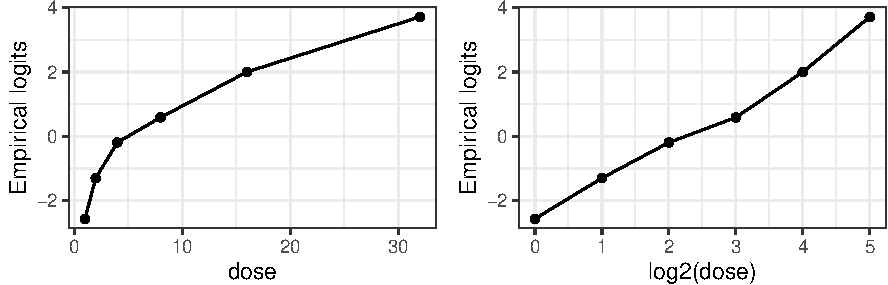
\includegraphics{rcas_files/figure-latex/budworm-1.pdf}
\caption{\label{fig:budworm}Insecticide mortality of the moth tobacco
budworm.}
\end{figure}

\hypertarget{sec:logistic-each-component}{%
\subsubsection{Each component of the
likelihood}\label{sec:logistic-each-component}}

The log-likelihood is
\(\log L=\sum_i y_i \log(p_i) + (n_i-y_i) \log(1-p_i) = \sum_i \log L_i\),
say. With \(\log(p_i/(1-p_i)) = s_i\) we have
\(p_i=1 / (1+ \exp(-s_i))\) and
\(\frac d {ds_i} p_i = \frac{\exp(- s_i)}{\left(1 + \exp(- s_i)\right)^{2}}\).
With \(s_i = x_i\cdot b\), we have \(\frac d {db} s_i = x_i\).

Consider the contribution to the total log-likelihood from the \(i\)th
observation which is \(l_i = y_i \log(p_i) + (n_i-y_i) \log(1-p_i)\).
Since we are focusing on one observation only, we shall ignore the
subscript \(i\) in this section. The log-likelihood and its derivative
are:

\begin{Shaded}
\begin{Highlighting}[]
\NormalTok{R}\OperatorTok{>}\StringTok{ }\KeywordTok{def_sym}\NormalTok{(y, n, p, x, s, b)}
\NormalTok{R}\OperatorTok{>}\StringTok{ }\NormalTok{logL_ <-}\StringTok{ }\NormalTok{y }\OperatorTok{*}\StringTok{ }\KeywordTok{log}\NormalTok{(p) }\OperatorTok{+}\StringTok{ }\NormalTok{(n }\OperatorTok{-}\StringTok{ }\NormalTok{y) }\OperatorTok{*}\StringTok{ }\KeywordTok{log}\NormalTok{(}\DecValTok{1} \OperatorTok{-}\StringTok{ }\NormalTok{p)}
\NormalTok{R}\OperatorTok{>}\StringTok{ }\NormalTok{gp_ <-}\StringTok{ }\KeywordTok{der}\NormalTok{(logL_, p)}
\NormalTok{R}\OperatorTok{>}\StringTok{ }\NormalTok{gp_}
\end{Highlighting}
\end{Shaded}

\begin{verbatim}
## c:   n - y   y
##    - ----- + -
##      1 - p   p
\end{verbatim}

The underscore in \texttt{logL\_} and elsewhere indicates that this
expression is defined in terms of other symbols. This is in contrast to
the free variables, e.g.~\texttt{y}, \texttt{p}, and \texttt{n}. With
\(s = \log(p/(1-p))\) we can find \(p\) as:

\begin{Shaded}
\begin{Highlighting}[]
\NormalTok{R}\OperatorTok{>}\StringTok{ }\NormalTok{sol_ <-}\StringTok{ }\KeywordTok{solve_sys}\NormalTok{(}\KeywordTok{log}\NormalTok{(p }\OperatorTok{/}\StringTok{ }\NormalTok{(}\DecValTok{1} \OperatorTok{-}\StringTok{ }\NormalTok{p)), s, p)}
\NormalTok{R}\OperatorTok{>}\StringTok{ }\NormalTok{p_ <-}\StringTok{ }\NormalTok{sol_[[}\DecValTok{1}\NormalTok{]]}\OperatorTok{$}\NormalTok{p}
\NormalTok{R}\OperatorTok{>}\StringTok{ }\NormalTok{p_}
\end{Highlighting}
\end{Shaded}

\begin{verbatim}
## c:   exp(s)  
##    ----------
##    exp(s) + 1
\end{verbatim}

The log-likelihood and its derivative as functions of \(s\) become:

\begin{Shaded}
\begin{Highlighting}[]
\NormalTok{R}\OperatorTok{>}\StringTok{ }\NormalTok{logL2_ <-}\StringTok{ }\KeywordTok{subs}\NormalTok{(logL_, p, p_)}
\NormalTok{R}\OperatorTok{>}\StringTok{ }\NormalTok{logL2_}
\end{Highlighting}
\end{Shaded}

\begin{verbatim}
## c:      /  exp(s)  \              /      exp(s)  \
##    y*log|----------| + (n - y)*log|1 - ----------|
##         \exp(s) + 1/              \    exp(s) + 1/
\end{verbatim}

\begin{Shaded}
\begin{Highlighting}[]
\NormalTok{R}\OperatorTok{>}\StringTok{ }\NormalTok{gs_ <-}\StringTok{ }\KeywordTok{der}\NormalTok{(logL2_, s) }\OperatorTok{|}\ErrorTok{>}\StringTok{ }\KeywordTok{simplify}\NormalTok{()}
\NormalTok{R}\OperatorTok{>}\StringTok{ }\NormalTok{gs_}
\end{Highlighting}
\end{Shaded}

\begin{verbatim}
## c: -n*exp(s) + y*exp(s) + y
##    ------------------------
##           exp(s) + 1
\end{verbatim}

Lastly we connect \(s\) to the regression coefficients \(b\) and compute
the score function, \(S\), and the Hessian, \(H\):

\begin{Shaded}
\begin{Highlighting}[]
\NormalTok{R}\OperatorTok{>}\StringTok{ }\NormalTok{s_ <-}\StringTok{ }\KeywordTok{sum}\NormalTok{(x }\OperatorTok{*}\StringTok{ }\NormalTok{b)}
\NormalTok{R}\OperatorTok{>}\StringTok{ }\NormalTok{logL3_ <-}\StringTok{ }\KeywordTok{subs}\NormalTok{(logL2_, s, s_)}
\end{Highlighting}
\end{Shaded}

\begin{Shaded}
\begin{Highlighting}[]
\NormalTok{R}\OperatorTok{>}\StringTok{ }\NormalTok{S_ <-}\StringTok{ }\KeywordTok{score}\NormalTok{(logL3_, b) }\OperatorTok{|}\ErrorTok{>}\StringTok{ }\KeywordTok{simplify}\NormalTok{()}
\NormalTok{R}\OperatorTok{>}\StringTok{ }\NormalTok{H_ <-}\StringTok{ }\KeywordTok{hessian}\NormalTok{(logL3_, b) }\OperatorTok{|}\ErrorTok{>}\StringTok{ }\KeywordTok{simplify}\NormalTok{()}
\NormalTok{R}\OperatorTok{>}\StringTok{ }\NormalTok{S_}
\end{Highlighting}
\end{Shaded}

\begin{verbatim}
## c: [x*(y - (n - y)*exp(b*x))]
##    [------------------------]
##    [      exp(b*x) + 1      ]
\end{verbatim}

\begin{Shaded}
\begin{Highlighting}[]
\NormalTok{R}\OperatorTok{>}\StringTok{ }\NormalTok{H_}
\end{Highlighting}
\end{Shaded}

\begin{verbatim}
## c: [          2                ]
##    [      -n*x *exp(b*x)       ]
##    [---------------------------]
##    [exp(2*b*x) + 2*exp(b*x) + 1]
\end{verbatim}

Since \(x\) and \({b}\) are vectors, the term \texttt{x*b} above should
be read as the inner product \(x \cdot {b}\) (or as \(x^\top{b}\) in
matrix notation). Also, since \(x\) is a vector, the term
\texttt{x\^{}2} above should be read as the outer product
\(x \otimes x\) (or as \(x x^\top\) in matrix notation). More insight in
the structure is obtained by letting \(b\) and \(x\) be \(2\)-vectors.
(to save space, only the score function is shown in the following):

\begin{Shaded}
\begin{Highlighting}[]
\NormalTok{R}\OperatorTok{>}\StringTok{ }\NormalTok{b <-}\StringTok{ }\KeywordTok{vector_sym}\NormalTok{(}\DecValTok{2}\NormalTok{, }\StringTok{"b"}\NormalTok{)}
\NormalTok{R}\OperatorTok{>}\StringTok{ }\NormalTok{x <-}\StringTok{ }\KeywordTok{vector_sym}\NormalTok{(}\DecValTok{2}\NormalTok{, }\StringTok{"x"}\NormalTok{)}
\NormalTok{R}\OperatorTok{>}\StringTok{ }\NormalTok{s_ <-}\StringTok{ }\KeywordTok{sum}\NormalTok{(x }\OperatorTok{*}\StringTok{ }\NormalTok{b)}
\NormalTok{R}\OperatorTok{>}\StringTok{ }\NormalTok{logL3_ <-}\StringTok{ }\KeywordTok{subs}\NormalTok{(logL2_, s, s_)}
\end{Highlighting}
\end{Shaded}

Again, we compute the score function \(S\) by differentiation with
respect to the regression parameters. This gives a vector valued funtion
of the regression parameters and data.

\begin{Shaded}
\begin{Highlighting}[]
\NormalTok{R}\OperatorTok{>}\StringTok{ }\NormalTok{S_ <-}\StringTok{ }\KeywordTok{score}\NormalTok{(logL3_, b) }\OperatorTok{|}\ErrorTok{>}\StringTok{ }\KeywordTok{simplify}\NormalTok{()}
\end{Highlighting}
\end{Shaded}

Next, insert data, e.g.~\(x_{1}=1\), \(x_{2}=2\), \(y=9\), \(n=20\) to
obtain a function of the regression parameters only:

\begin{Shaded}
\begin{Highlighting}[]
\NormalTok{R}\OperatorTok{>}\StringTok{ }\NormalTok{nms <-}\StringTok{ }\KeywordTok{c}\NormalTok{(}\StringTok{"x1"}\NormalTok{, }\StringTok{"x2"}\NormalTok{, }\StringTok{"y"}\NormalTok{, }\StringTok{"n"}\NormalTok{)}
\NormalTok{R}\OperatorTok{>}\StringTok{ }\NormalTok{vls <-}\StringTok{ }\KeywordTok{c}\NormalTok{(}\DecValTok{1}\NormalTok{, }\DecValTok{2}\NormalTok{, }\DecValTok{9}\NormalTok{, }\DecValTok{20}\NormalTok{)}
\NormalTok{R}\OperatorTok{>}\StringTok{ }\NormalTok{S. <-}\StringTok{ }\KeywordTok{subs}\NormalTok{(S_, nms, vls)}
\end{Highlighting}
\end{Shaded}

Note how the expression depending on other symbols, \texttt{S\_}, is
named \texttt{S.} to indiciate that data has been inserted:

\begin{align}
\texttt{S\_} = \left[\begin{matrix}[r]\frac{x_{1} \left(- n e^{b_{1} x_{1} + b_{2} x_{2}} + y e^{b_{1} x_{1} + b_{2} x_{2}} + y\right)}{e^{b_{1} x_{1} + b_{2} x_{2}} + 1}\\\frac{x_{2} \left(- n e^{b_{1} x_{1} + b_{2} x_{2}} + y e^{b_{1} x_{1} + b_{2} x_{2}} + y\right)}{e^{b_{1} x_{1} + b_{2} x_{2}} + 1}\end{matrix}\right], \quad S. = \left[\begin{matrix}[r]\frac{9 - 11 e^{b_{1} + 2 b_{2}}}{e^{b_{1} + 2 b_{2}} + 1}\\\frac{2 \left(9 - 11 e^{b_{1} + 2 b_{2}}\right)}{e^{b_{1} + 2 b_{2}} + 1}\end{matrix}\right]
\end{align}

An alternative is to create \texttt{R}\ functions and subsequently set
default values

\begin{Shaded}
\begin{Highlighting}[]
\NormalTok{R}\OperatorTok{>}\StringTok{ }\NormalTok{S.. <-}\StringTok{ }\KeywordTok{as_func}\NormalTok{(S_, }\DataTypeTok{order =} \KeywordTok{c}\NormalTok{(}\StringTok{"b1"}\NormalTok{, }\StringTok{"b2"}\NormalTok{, }\StringTok{"x1"}\NormalTok{, }\StringTok{"x2"}\NormalTok{, }\StringTok{"y"}\NormalTok{, }\StringTok{"n"}\NormalTok{))}
\NormalTok{R}\OperatorTok{>}\StringTok{ }\NormalTok{S... <-}\StringTok{ }\ControlFlowTok{function}\NormalTok{(b1, b2) \{}
\OperatorTok{+}\StringTok{   }\KeywordTok{S..}\NormalTok{(b1, b2, }\DataTypeTok{x1 =}\NormalTok{ vls[}\DecValTok{1}\NormalTok{], }\DataTypeTok{x2 =}\NormalTok{ vls[}\DecValTok{2}\NormalTok{], }\DataTypeTok{y =}\NormalTok{ vls[}\DecValTok{3}\NormalTok{], }\DataTypeTok{n =}\NormalTok{ vls[}\DecValTok{4}\NormalTok{])}
\OperatorTok{+}\StringTok{ }\NormalTok{\}}
\NormalTok{R}\OperatorTok{>}\StringTok{ }\KeywordTok{S...}\NormalTok{(}\DecValTok{1}\NormalTok{, }\DecValTok{1}\NormalTok{)}
\end{Highlighting}
\end{Shaded}

\begin{verbatim}
##       [,1]
## [1,] -10.1
## [2,] -20.1
\end{verbatim}

\hypertarget{the-total-likelihood-numerically}{%
\subsubsection{The total likelihood
numerically}\label{the-total-likelihood-numerically}}

The score and Hessian for a full data set is the sum of such terms and
it is a straight forward \texttt{R} task to construct these sums. In
either case the result is a function of the regression coefficients
which can be used in connection with numerical optimization. This could
be a Newton-Rapson algorithm (which would also require the Hessian as
function) or a coordinate descent or similar method.

\begin{Shaded}
\begin{Highlighting}[]
\NormalTok{R}\OperatorTok{>}\StringTok{ }\NormalTok{Sv <-}\StringTok{ }\KeywordTok{Vectorize}\NormalTok{(S.., }\DataTypeTok{vectorize.args =} \KeywordTok{c}\NormalTok{(}\StringTok{"x1"}\NormalTok{, }\StringTok{"x2"}\NormalTok{, }\StringTok{"y"}\NormalTok{, }\StringTok{"n"}\NormalTok{))}
\NormalTok{R}\OperatorTok{>}\StringTok{ }\NormalTok{Sv_wrap <-}\StringTok{ }\ControlFlowTok{function}\NormalTok{(b1, b2) \{}
\OperatorTok{+}\StringTok{   }\KeywordTok{Sv}\NormalTok{(b1, b2, }\DataTypeTok{x1 =} \KeywordTok{rep}\NormalTok{(}\DecValTok{1}\NormalTok{, }\KeywordTok{nrow}\NormalTok{(bud)), }\DataTypeTok{x2 =} \KeywordTok{log2}\NormalTok{(bud}\OperatorTok{$}\NormalTok{dose), }\DataTypeTok{y =}\NormalTok{ bud}\OperatorTok{$}\NormalTok{ndead, }\DataTypeTok{n =}\NormalTok{ bud}\OperatorTok{$}\NormalTok{ntotal)}
\OperatorTok{+}\StringTok{ }\NormalTok{\}}
\NormalTok{R}\OperatorTok{>}\StringTok{ }\KeywordTok{Sv_wrap}\NormalTok{(}\DecValTok{1}\NormalTok{, }\DecValTok{1}\NormalTok{)}
\end{Highlighting}
\end{Shaded}

\begin{verbatim}
##       [,1]  [,2]  [,3]   [,4]  [,5]   [,6]
## [1,] -13.6 -13.6 -10.1  -6.64 -1.87 0.0495
## [2,]   0.0 -13.6 -20.1 -19.92 -7.46 0.2473
\end{verbatim}

\begin{Shaded}
\begin{Highlighting}[]
\NormalTok{R}\OperatorTok{>}\StringTok{ }\KeywordTok{apply}\NormalTok{(}\KeywordTok{Sv_wrap}\NormalTok{(}\DecValTok{1}\NormalTok{, }\DecValTok{1}\NormalTok{), }\DecValTok{1}\NormalTok{, sum)}
\end{Highlighting}
\end{Shaded}

\begin{verbatim}
## [1] -45.7 -60.9
\end{verbatim}

\begin{Shaded}
\begin{Highlighting}[]
\NormalTok{R}\OperatorTok{>}\StringTok{ }\KeywordTok{apply}\NormalTok{(}\KeywordTok{Sv_wrap}\NormalTok{(}\DecValTok{2}\NormalTok{, }\DecValTok{2}\NormalTok{), }\DecValTok{1}\NormalTok{, sum)}
\end{Highlighting}
\end{Shaded}

\begin{verbatim}
## [1] -52.2 -66.5
\end{verbatim}

\hypertarget{sec:logistic-all-likelihood}{%
\subsubsection{The total likelihood
symbolically}\label{sec:logistic-all-likelihood}}

An alternative to the approach above is to specify the full likelihood
directly:

\begin{Shaded}
\begin{Highlighting}[]
\NormalTok{R}\OperatorTok{>}\StringTok{ }\NormalTok{N <-}\StringTok{ }\DecValTok{6} \CommentTok{## Number of rows in dataset}
\NormalTok{R}\OperatorTok{>}\StringTok{ }\NormalTok{q <-}\StringTok{ }\DecValTok{2} \CommentTok{## Number of explanatory variables}
\NormalTok{R}\OperatorTok{>}\StringTok{ }\NormalTok{X <-}\StringTok{ }\KeywordTok{matrix_sym}\NormalTok{(N, q, }\StringTok{"x"}\NormalTok{)}
\NormalTok{R}\OperatorTok{>}\StringTok{ }\NormalTok{y <-}\StringTok{ }\KeywordTok{vector_sym}\NormalTok{(N, }\StringTok{"y"}\NormalTok{)}
\NormalTok{R}\OperatorTok{>}\StringTok{ }\NormalTok{n <-}\StringTok{ }\KeywordTok{vector_sym}\NormalTok{(N, }\StringTok{"n"}\NormalTok{)}
\NormalTok{R}\OperatorTok{>}\StringTok{ }\NormalTok{p <-}\StringTok{ }\KeywordTok{vector_sym}\NormalTok{(N, }\StringTok{"p"}\NormalTok{)}
\NormalTok{R}\OperatorTok{>}\StringTok{ }\NormalTok{s <-}\StringTok{ }\KeywordTok{vector_sym}\NormalTok{(N, }\StringTok{"s"}\NormalTok{)}
\NormalTok{R}\OperatorTok{>}\StringTok{ }\NormalTok{b <-}\StringTok{ }\KeywordTok{vector_sym}\NormalTok{(q, }\StringTok{"b"}\NormalTok{)}
\end{Highlighting}
\end{Shaded}

\[
 X=\left[\begin{matrix}[r]x_{11} & x_{12}\\x_{21} & x_{22}\\x_{31} & x_{32}\\x_{41} & x_{42}\\x_{51} & x_{52}\\x_{61} & x_{62}\end{matrix}\right], \quad
 n=\left[\begin{matrix}[r]n_{1}\\n_{2}\\n_{3}\\n_{4}\\n_{5}\\n_{6}\end{matrix}\right], \quad
 y=\left[\begin{matrix}[r]y_{1}\\y_{2}\\y_{3}\\y_{4}\\y_{5}\\y_{6}\end{matrix}\right]
\]

The symbolic computations are as follows:

\begin{Shaded}
\begin{Highlighting}[]
\NormalTok{R}\OperatorTok{>}\StringTok{ }\CommentTok{## log-likelihood:}
\NormalTok{R}\OperatorTok{>}\StringTok{ }\NormalTok{logL_  <-}\StringTok{ }\KeywordTok{sum}\NormalTok{(y }\OperatorTok{*}\StringTok{ }\KeywordTok{log}\NormalTok{(p) }\OperatorTok{+}\StringTok{ }\NormalTok{(n}\OperatorTok{-}\NormalTok{y) }\OperatorTok{*}\StringTok{ }\KeywordTok{log}\NormalTok{(}\DecValTok{1}\OperatorTok{-}\NormalTok{p))}
\NormalTok{R}\OperatorTok{>}\StringTok{ }\CommentTok{## connecting p and s:}
\NormalTok{R}\OperatorTok{>}\StringTok{ }\NormalTok{p_ <-}\StringTok{ }\DecValTok{1} \OperatorTok{/}\StringTok{ }\NormalTok{(}\DecValTok{1} \OperatorTok{+}\StringTok{ }\KeywordTok{exp}\NormalTok{(}\OperatorTok{-}\NormalTok{s))}
\NormalTok{R}\OperatorTok{>}\StringTok{ }\CommentTok{## log-likelihood as function of linear predictor:}
\NormalTok{R}\OperatorTok{>}\StringTok{ }\NormalTok{logL2_ <-}\StringTok{ }\KeywordTok{subs}\NormalTok{(logL_, p, p_)}
\NormalTok{R}\OperatorTok{>}\StringTok{ }\CommentTok{## linear predictor as function of regression coefficients:}
\NormalTok{R}\OperatorTok{>}\StringTok{ }\NormalTok{s_  <-}\StringTok{ }\NormalTok{X }\OperatorTok\StringTok{ }\NormalTok{b}
\NormalTok{R}\OperatorTok{>}\StringTok{ }\CommentTok{## log-Likelihood as function of regression coefficients:}
\NormalTok{R}\OperatorTok{>}\StringTok{ }\NormalTok{logL3_ <-}\StringTok{ }\KeywordTok{subs}\NormalTok{(logL2_, s, s_)}
\NormalTok{R}\OperatorTok{>}\StringTok{ }\CommentTok{## Score and Hessian:}
\NormalTok{R}\OperatorTok{>}\StringTok{ }\NormalTok{S_ <-}\StringTok{ }\KeywordTok{score}\NormalTok{(logL3_, b) }
\NormalTok{R}\OperatorTok{>}\StringTok{ }\NormalTok{H_ <-}\StringTok{ }\KeywordTok{hessian}\NormalTok{(logL3_, b)}
\end{Highlighting}
\end{Shaded}

Above we have analysed the logistic regression model with the logit
link. If we instead used the complementary log log link,
\(\eta = \log(-\log(1-p))\) and find the inverse

\begin{Shaded}
\begin{Highlighting}[]
\NormalTok{R}\OperatorTok{>}\StringTok{ }\NormalTok{sol_ <-}\StringTok{ }\KeywordTok{solve_sys}\NormalTok{(}\KeywordTok{log}\NormalTok{(}\OperatorTok{-}\KeywordTok{log}\NormalTok{(}\DecValTok{1}\OperatorTok{-}\NormalTok{p)), s, p)}
\NormalTok{R}\OperatorTok{>}\StringTok{ }\NormalTok{sol_}
\end{Highlighting}
\end{Shaded}

which can be used in the above by specifying

\begin{Shaded}
\begin{Highlighting}[]
\NormalTok{R}\OperatorTok{>}\StringTok{ }\NormalTok{p_ <-}\StringTok{ }\DecValTok{1} \OperatorTok{-}\StringTok{ }\KeywordTok{exp}\NormalTok{(}\OperatorTok{-}\KeywordTok{exp}\NormalTok{(s))}
\end{Highlighting}
\end{Shaded}

{[}FIXME: SH: Above{]}

\hypertarget{sec:ar1}{%
\subsection{Auto regressive models}\label{sec:ar1}}

\hypertarget{an-ar1-model}{%
\subsubsection{\texorpdfstring{An \(AR(1)\)
model}{An AR(1) model}}\label{an-ar1-model}}

In this section we study the auto regressive model of order \(1\) (an
AR(1) model), see e.g.~\citep{shumway:etal:16}, p.~75 ff.~for details:
Consider random variables \(x_1, x_2, \dots, x_n\) following a
stationary zero mean AR(1) process

\begin{equation}
  \label{eq:ar1}
  x_i = a x_{i-1} + e_i; \quad i=2, \dots, n
\end{equation}

where \(e_i \sim N(0, v)\) and all \(e_i\)s are independent. Note that
\(v\) denotes the variance. The marginal distribution of \(x_1\) is also
assumed normal, and for the process to be stationary we must have
\(\mathbf{Var}(x_1) = v / (1-a^2)\). Hence we can write
\(x_1 = \frac 1 {\sqrt{1-a^2}} e_1\).

For simplicity of exposition, we set \(n=4\). All terms
\(e_1, \dots, e_4\) are independent and \(N(0, v)\) distributed. Let
\(e=(e_1, \dots, e_4)\) and \(x=(x_1, \dots x_4)\). Hence
\(e \sim N(0, v I)\). Isolating error terms gives

\begin{displaymath}
  e= \left[\begin{matrix}e_{1}\\e_{2}\\e_{3}\\e_{4}\end{matrix}\right] = \left[\begin{matrix}[r]\sqrt{1 - a^{2}} & . & . & .\\- a & 1 & . & .\\. & - a & 1 & .\\. & . & - a & 1\end{matrix}\right] \left[\begin{matrix}x_{1}\\x_{2}\\x_{3}\\x_{4}\end{matrix}\right] = L x 
\end{displaymath}

Since \(\mathbf{Var}(e)=v I\) we have
\(\mathbf{Var}(e)=v I=L \mathbf{Var}(x) L'\) so the covariance matrix of
\(x\) is \(V=\mathbf{Var}(x) = v L^- (L^-)^\top\) while the
concentration matrix (the inverse covariances matrix) is
\(K=v^{-1}L^\top L\).

\begin{Shaded}
\begin{Highlighting}[]
\NormalTok{R}\OperatorTok{>}\StringTok{ }\NormalTok{n <-}\StringTok{ }\DecValTok{4}
\NormalTok{R}\OperatorTok{>}\StringTok{ }\KeywordTok{def_sym}\NormalTok{(a)}
\NormalTok{R}\OperatorTok{>}\StringTok{ }\NormalTok{x <-}\StringTok{ }\KeywordTok{vector_sym}\NormalTok{(n, }\StringTok{"x"}\NormalTok{)}
\NormalTok{R}\OperatorTok{>}\StringTok{ }\NormalTok{e <-}\StringTok{ }\KeywordTok{vector_sym}\NormalTok{(n, }\StringTok{"e"}\NormalTok{)}
\NormalTok{R}\OperatorTok{>}\StringTok{ }\NormalTok{L <-}\StringTok{ }\KeywordTok{diff_mat}\NormalTok{(n, }\StringTok{"-a"}\NormalTok{)}
\NormalTok{R}\OperatorTok{>}\StringTok{ }\NormalTok{L[}\DecValTok{1}\NormalTok{, }\DecValTok{1}\NormalTok{] <-}\StringTok{ }\KeywordTok{sqrt}\NormalTok{(}\DecValTok{1}\OperatorTok{-}\NormalTok{a}\OperatorTok{^}\DecValTok{2}\NormalTok{)}
\end{Highlighting}
\end{Shaded}

\begin{Shaded}
\begin{Highlighting}[]
\NormalTok{R}\OperatorTok{>}\StringTok{ }\KeywordTok{def_sym}\NormalTok{(v)}
\NormalTok{R}\OperatorTok{>}\StringTok{ }\NormalTok{Linv <-}\StringTok{ }\KeywordTok{inv}\NormalTok{(L)}
\NormalTok{R}\OperatorTok{>}\StringTok{ }\NormalTok{K <-}\StringTok{ }\KeywordTok{crossprod_}\NormalTok{(L) }\OperatorTok{/}\StringTok{ }\NormalTok{v}
\NormalTok{R}\OperatorTok{>}\StringTok{ }\NormalTok{V <-}\StringTok{ }\KeywordTok{tcrossprod_}\NormalTok{(Linv) }\OperatorTok{*}\StringTok{ }\NormalTok{v}
\end{Highlighting}
\end{Shaded}

\begin{align} 
    L^{-1}&= \left[\begin{matrix}[r]\frac{1}{\sqrt{1 - a^{2}}} & . & . & .\\\frac{a}{\sqrt{1 - a^{2}}} & 1 & . & .\\\frac{a^{2}}{\sqrt{1 - a^{2}}} & a & 1 & .\\\frac{a^{3}}{\sqrt{1 - a^{2}}} & a^{2} & a & 1\end{matrix}\right] \\ 
    K &= \frac{1}{v}  \left[\begin{matrix}[r]1 & - a & . & .\\- a & a^{2} + 1 & - a & .\\. & - a & a^{2} + 1 & - a\\. & . & - a & 1\end{matrix}\right] \\ 
    V &= v  \left[\begin{matrix}[r]\frac{1}{1 - a^{2}} & \frac{a}{1 - a^{2}} & \frac{a^{2}}{1 - a^{2}} & \frac{a^{3}}{1 - a^{2}}\\\frac{a}{1 - a^{2}} & \frac{a^{2}}{1 - a^{2}} + 1 & \frac{a^{3}}{1 - a^{2}} + a & \frac{a^{4}}{1 - a^{2}} + a^{2}\\\frac{a^{2}}{1 - a^{2}} & \frac{a^{3}}{1 - a^{2}} + a & \frac{a^{4}}{1 - a^{2}} + a^{2} + 1 & \frac{a^{5}}{1 - a^{2}} + a^{3} + a\\\frac{a^{3}}{1 - a^{2}} & \frac{a^{4}}{1 - a^{2}} + a^{2} & \frac{a^{5}}{1 - a^{2}} + a^{3} + a & \frac{a^{6}}{1 - a^{2}} + a^{4} + a^{2} + 1\end{matrix}\right] 
  \end{align}

The zeros in the concentration matrix \(K\) implies a conditional
independence restrstriction: If the \(ij\)th element of a concentration
matrix is zero then \(x_i\) and \(x_j\) are conditionally independent
given all other variables, see e.g.~\citep{hojsgaard:etal:12}, chap.~4
for details.\footnote{BETTER REFERENCE; Handbook of graphical models
perhaps?}

Next, we take the step from symbolic computations to numerical
evaluations. The joint distribution of \(x\) is multivariate normal
distribution, \(x\sim N(0, K^{-1})\). Let \(W=x x^\top\) denote the
matrix of (cross) products. The log-likelihood is therefore (ignoring
multiplicative constants) \[ 
\log L = \log \mathbf{det}(K) - x^\top K x = \log \mathbf{det}(K) - \mathbf{tr}(K W), 
\] where we note that \(\mathbf{tr}(KW)\) is the sum of the elementwise
products of \(K\) and \(W\) since both matrices are symmetrical.

\begin{Shaded}
\begin{Highlighting}[]
\NormalTok{R}\OperatorTok{>}\StringTok{ }\NormalTok{logL <-}\StringTok{ }\KeywordTok{log}\NormalTok{(}\KeywordTok{det}\NormalTok{(K)) }\OperatorTok{-}\StringTok{ }\KeywordTok{sum}\NormalTok{(K }\OperatorTok{*}\StringTok{ }\NormalTok{(x }\OperatorTok\StringTok{ }\KeywordTok{t}\NormalTok{(x))) }\OperatorTok\StringTok{ }\KeywordTok{simplify}\NormalTok{()}
\end{Highlighting}
\end{Shaded}

\[
\log L = \log{\left(- \frac{a^{2}}{v^{4}} + \frac{1}{v^{4}} \right)} - \frac{- 2 a x_{1} x_{2} - 2 a x_{2} x_{3} - 2 a x_{3} x_{4} + x_{1}^{2} + x_{2}^{2} \left(a^{2} + 1\right) + x_{3}^{2} \left(a^{2} + 1\right) + x_{4}^{2}}{v}
\]

\hypertarget{bridging-the-gap---towards-numerical-evaluation}{%
\subsubsection{Bridging the gap - towards numerical
evaluation}\label{bridging-the-gap---towards-numerical-evaluation}}

Next we illustrate how bridge the gap from symbolic computations to
numerical computations based on a dataset: For a specific data vector we
get

\begin{Shaded}
\begin{Highlighting}[]
\NormalTok{R}\OperatorTok{>}\StringTok{ }\NormalTok{xt <-}\StringTok{ }\KeywordTok{c}\NormalTok{(}\FloatTok{0.1}\NormalTok{, }\FloatTok{-0.9}\NormalTok{, }\FloatTok{0.4}\NormalTok{, }\FloatTok{.0}\NormalTok{)}
\NormalTok{R}\OperatorTok{>}\StringTok{ }\NormalTok{logL. <-}\StringTok{ }\KeywordTok{subs}\NormalTok{(logL, x, xt) }
\end{Highlighting}
\end{Shaded}

\[
\log L = \log{\left(- \frac{a^{2}}{v^{4}} + \frac{1}{v^{4}} \right)} - \frac{0.97 a^{2} + 0.9 a + 0.98}{v}
\]

We can use \texttt{R}\ for numerical maximization of the likelihood and
constraints on the parameter values can be imposed e.g.~in the
\texttt{optim()} function:

\begin{Shaded}
\begin{Highlighting}[]
\NormalTok{R}\OperatorTok{>}\StringTok{ }\NormalTok{f_wrap <-}\StringTok{ }\KeywordTok{as_func}\NormalTok{(logL., }\DataTypeTok{vec_arg =} \OtherTok{TRUE}\NormalTok{)}
\NormalTok{R}\OperatorTok{>}\StringTok{ }\NormalTok{eps <-}\StringTok{ }\FloatTok{0.01}
\NormalTok{R}\OperatorTok{>}\StringTok{ }\NormalTok{par <-}\StringTok{ }\KeywordTok{optim}\NormalTok{(}\KeywordTok{c}\NormalTok{(}\DataTypeTok{a=}\DecValTok{0}\NormalTok{, }\DataTypeTok{v=}\DecValTok{1}\NormalTok{), f_wrap, }\DataTypeTok{lower=}\KeywordTok{c}\NormalTok{(}\OperatorTok{-}\NormalTok{(}\DecValTok{1}\OperatorTok{-}\NormalTok{eps), eps), }\DataTypeTok{upper=}\KeywordTok{c}\NormalTok{((}\DecValTok{1}\OperatorTok{-}\NormalTok{eps), }\DecValTok{10}\NormalTok{),}
\OperatorTok{+}\StringTok{              }\DataTypeTok{method=}\StringTok{"L-BFGS-B"}\NormalTok{, }\DataTypeTok{control=}\KeywordTok{list}\NormalTok{(}\DataTypeTok{fnscale=}\OperatorTok{-}\DecValTok{1}\NormalTok{))}\OperatorTok{$}\NormalTok{par}
\NormalTok{R}\OperatorTok{>}\StringTok{ }\NormalTok{par}
\end{Highlighting}
\end{Shaded}

\begin{verbatim}
##      a      v 
## -0.376  0.195
\end{verbatim}

The same model can be fitted e.g.~using \texttt{R}'s \texttt{arima()}
function as follows (output omitted):

\begin{Shaded}
\begin{Highlighting}[]
\NormalTok{R}\OperatorTok{>}\StringTok{ }\KeywordTok{arima}\NormalTok{(xt, }\DataTypeTok{order =} \KeywordTok{c}\NormalTok{(}\DecValTok{1}\NormalTok{, }\DecValTok{0}\NormalTok{, }\DecValTok{0}\NormalTok{), }\DataTypeTok{include.mean =} \OtherTok{FALSE}\NormalTok{, }\DataTypeTok{method =} \StringTok{"ML"}\NormalTok{)}
\end{Highlighting}
\end{Shaded}

It is less trivial to do the optimization in \texttt{caracas} by solving
the score equations. There are some possibilities for putting
assumptions on variables in \texttt{caracas} (see the ``Reference''
vignette), but it is not possible to restrict variables to only take
values in \((-1, 1)\).

\hypertarget{sec:cont_tab}{%
\subsection{Maximum likelihood under constraints - independence model
for two-way contingency table}\label{sec:cont_tab}}

In this section we illustrate constrained optimization using Lagrange
multipliers. Consider a \(2 \times 2\) contingency table with cell
counts \(n_{ij}\) and cell probabilities \(p_{ij}\) for \(i=1,2\) and
\(j=1,2\).

\begin{verbatim}
##    c
## r   1   2  
##   1 n11 n12
##   2 n21 n22
\end{verbatim}

Under multinomial sampling, the log likelihood is \[
 l = \log L = \sum_{ij} n_{ij} \log(p_{ij}).
\]

Under the assumption of independence between rows and columns, the cell
probabilities have the form, (see e.g.~{[}REFERENCE{]}, chap.~XXX) \[
p_{ij}=u r_i s_j.
\]

To make the parameters \((u, r_i, s_j)\) identifiable, constraints must
be imposed. One possibility is to require that \(r_1=s_1=1\). The task
is then to estimate \(u\), \(r_2\), \(s_2\) by maximizing the log
likelihood under the constraint that \(\sum_{ij} p_{ij} = 1\). This can
be achieved using a Lagrange multiplier where we instead solve the
unconstrained optimization problem \(\max_p Lag(p)\) where \begin{align}
  Lag(p) &= -l(p) + \lambda g(p) \quad \text{under the constraint that} \\
  g(p) &= \sum_{ij} p_{ij} - 1 = 0.
\end{align} where \(\lambda\) is a Lagrange multiplier.

\begin{Shaded}
\begin{Highlighting}[]
\NormalTok{R}\OperatorTok{>}\StringTok{ }\NormalTok{n_ <-}\StringTok{ }\KeywordTok{c}\NormalTok{(}\StringTok{"n11"}\NormalTok{, }\StringTok{"n21"}\NormalTok{, }\StringTok{"n12"}\NormalTok{, }\StringTok{"n22"}\NormalTok{)}
\NormalTok{R}\OperatorTok{>}\StringTok{ }\NormalTok{n  <-}\StringTok{ }\KeywordTok{as_sym}\NormalTok{(n_)}
\NormalTok{R}\OperatorTok{>}\StringTok{ }\KeywordTok{def_sym}\NormalTok{(u, r2, s2, lam)}
\NormalTok{R}\OperatorTok{>}\StringTok{ }\NormalTok{p <-}\StringTok{ }\KeywordTok{as_sym}\NormalTok{(}\KeywordTok{c}\NormalTok{(}\StringTok{"u"}\NormalTok{, }\StringTok{"u*r2"}\NormalTok{, }\StringTok{"u*s2"}\NormalTok{, }\StringTok{"u*r2*s2"}\NormalTok{))}
\NormalTok{R}\OperatorTok{>}\StringTok{ }\NormalTok{logL  <-}\StringTok{ }\KeywordTok{sum}\NormalTok{(n }\OperatorTok{*}\StringTok{ }\KeywordTok{log}\NormalTok{(p))}
\NormalTok{R}\OperatorTok{>}\StringTok{ }\NormalTok{Lag  <-}\StringTok{ }\OperatorTok{-}\NormalTok{logL }\OperatorTok{+}\StringTok{ }\NormalTok{lam }\OperatorTok{*}\StringTok{ }\NormalTok{(}\KeywordTok{sum}\NormalTok{(p) }\OperatorTok{-}\StringTok{ }\DecValTok{1}\NormalTok{) }
\NormalTok{R}\OperatorTok{>}\StringTok{ }\NormalTok{vars <-}\StringTok{ }\KeywordTok{list}\NormalTok{(u, r2, s2, lam)}
\NormalTok{R}\OperatorTok{>}\StringTok{ }\NormalTok{gLag <-}\StringTok{ }\KeywordTok{der}\NormalTok{(Lag, vars)}
\NormalTok{R}\OperatorTok{>}\StringTok{ }\NormalTok{sol <-}\StringTok{ }\KeywordTok{solve_sys}\NormalTok{(}\KeywordTok{to_vector}\NormalTok{(gLag), vars)}
\NormalTok{R}\OperatorTok{>}\StringTok{ }\KeywordTok{print}\NormalTok{(sol, }\DataTypeTok{method =} \StringTok{"ascii"}\NormalTok{)}
\end{Highlighting}
\end{Shaded}

\begin{verbatim}
## Solution 1:
##   u   =  (n11 + n12)*(n11 + n21)/(n11 + n12 + n21 + n22)^2 
##   r2  =  (n21 + n22)/(n11 + n12) 
##   s2  =  (n12 + n22)/(n11 + n21) 
##   lam =  n11 + n12 + n21 + n22
\end{verbatim}

\begin{Shaded}
\begin{Highlighting}[]
\NormalTok{R}\OperatorTok{>}\StringTok{ }\NormalTok{sol <-}\StringTok{ }\NormalTok{sol[[}\DecValTok{1}\NormalTok{]]}
\end{Highlighting}
\end{Shaded}

There is only one critical point. Fitted cell probabilities
\(\hat p_{ij}\) are:

\begin{Shaded}
\begin{Highlighting}[]
\NormalTok{R}\OperatorTok{>}\StringTok{ }\NormalTok{p11 <-}\StringTok{ }\NormalTok{sol}\OperatorTok{$}\NormalTok{u}
\NormalTok{R}\OperatorTok{>}\StringTok{ }\NormalTok{p21 <-}\StringTok{ }\NormalTok{sol}\OperatorTok{$}\NormalTok{u }\OperatorTok{*}\StringTok{ }\NormalTok{sol}\OperatorTok{$}\NormalTok{r2}
\NormalTok{R}\OperatorTok{>}\StringTok{ }\NormalTok{p12 <-}\StringTok{ }\NormalTok{sol}\OperatorTok{$}\NormalTok{u }\OperatorTok{*}\StringTok{ }\NormalTok{sol}\OperatorTok{$}\NormalTok{s2}
\NormalTok{R}\OperatorTok{>}\StringTok{ }\NormalTok{p22 <-}\StringTok{ }\NormalTok{sol}\OperatorTok{$}\NormalTok{u }\OperatorTok{*}\StringTok{ }\NormalTok{sol}\OperatorTok{$}\NormalTok{r2 }\OperatorTok{*}\StringTok{ }\NormalTok{sol}\OperatorTok{$}\NormalTok{s2}
\NormalTok{R}\OperatorTok{>}\StringTok{ }\NormalTok{p.hat <-}\StringTok{ }\KeywordTok{matrix_}\NormalTok{(}\KeywordTok{c}\NormalTok{(p11, p21, p12, p22), }\DataTypeTok{nrow =} \DecValTok{2}\NormalTok{)}
\end{Highlighting}
\end{Shaded}

\[
\hat p = \frac{1}{\left(n_{11} + n_{12} + n_{21} + n_{22}\right)^{2}}  \left[\begin{matrix}\left(n_{11} + n_{12}\right) \left(n_{11} + n_{21}\right) & \left(n_{11} + n_{12}\right) \left(n_{12} + n_{22}\right)\\\left(n_{11} + n_{21}\right) \left(n_{21} + n_{22}\right) & \left(n_{12} + n_{22}\right) \left(n_{21} + n_{22}\right)\end{matrix}\right]
\]

To verify that the maximum likelihood estimate has been found, we
compute the Hessian matrix which is negative definite (the Hessian
matrix is diagonal so the eigenvalues are the diagonal entries and these
are all negative), output omitted:

\begin{Shaded}
\begin{Highlighting}[]
\NormalTok{R}\OperatorTok{>}\StringTok{ }\NormalTok{H <-}\StringTok{ }\KeywordTok{hessian}\NormalTok{(logL, }\KeywordTok{list}\NormalTok{(u, r2, s2)) }\OperatorTok{|}\ErrorTok{>}\StringTok{ }\KeywordTok{simplify}\NormalTok{()}
\end{Highlighting}
\end{Shaded}

\hypertarget{sec:cov_fun}{%
\subsection{A compound symmetry covariance
structure}\label{sec:cov_fun}}

Consider random variables \(x_1,\dots, x_n\) where
\(\mathbf{Var}(x_i)=v\) and \(\mathbf{Cov}(x_i, x_j)=v r\) for
\(i\not = j\), where \(0 \le r| \le1\). For \(n=3\), the covariance
matrix of \((x_1,\dots, x_n)\) is therefore

\begin{equation}
  \label{eq:1}
  V= v R = v \left[\begin{matrix}1 & r & r\\r & 1 & r\\r & r & 1\end{matrix}\right]. 
\end{equation}

Let \(\bar x = \sum_i x_i / n\) denote the average. Suppose interest is
in the variance of the average, \(\mathbf{Var}(\bar x)\), when \(n\)
goes to infinity. One approach is as follow: Let \(1\) denote an
\(n\)-vector of \(1\)'s and let \(V\) be an \(n \times n\) matrix with
\(v\) on the diagonal and \(v r\) outside the diagonal. Then
\(\mathbf{Var}(\bar x)=\frac 1 {n^2} 1^\top V 1\). The answer lies in
studying the limiting behaviour of this expression when
\(n\rightarrow \infty\) and \texttt{caracas} can not handle this
directly.

What can be done in \texttt{caracas} is the following: The variance of a
sum \(x. = \sum_i x_i\) is
\(\mathbf{Var}(x.) = \sum_i \mathbf{Var}(x_i) + 2 \sum_{ij:i<j} \mathbf{Cov}(x_i, x_j)\).
For the specific model, one must by hand find that \[
\mathbf{Var}(x.) = n v + 2 v r n (n-1) / 2 = n v (1 + r (n-1)),
\quad
  \mathbf{Var}(\bar x) = v (1 + (n-1)r)/n.
\]

\begin{Shaded}
\begin{Highlighting}[]
\NormalTok{R}\OperatorTok{>}\StringTok{ }\KeywordTok{def_sym}\NormalTok{(v, r, n) }
\NormalTok{R}\OperatorTok{>}\StringTok{ }\NormalTok{var_sum <-}\StringTok{ }\NormalTok{n }\OperatorTok{*}\StringTok{ }\NormalTok{v }\OperatorTok{*}\StringTok{ }\NormalTok{( }\DecValTok{1} \OperatorTok{+}\StringTok{ }\NormalTok{r }\OperatorTok{*}\StringTok{ }\NormalTok{(n }\OperatorTok{-}\StringTok{ }\DecValTok{1}\NormalTok{))}
\NormalTok{R}\OperatorTok{>}\StringTok{ }\NormalTok{var_avg <-}\StringTok{ }\NormalTok{var_sum }\OperatorTok{/}\StringTok{ }\NormalTok{n}\OperatorTok{^}\DecValTok{2}
\NormalTok{R}\OperatorTok{>}\StringTok{ }\NormalTok{var_avg }\OperatorTok\StringTok{ }\KeywordTok{simplify}\NormalTok{()}
\end{Highlighting}
\end{Shaded}

\begin{verbatim}
## c: v*(r*(n - 1) + 1)
##    -----------------
##            n
\end{verbatim}

Now we can study the limiting behaviour of the variance
\(\mathbf{Var}(\bar x)\) in different situations:

\begin{Shaded}
\begin{Highlighting}[]
\NormalTok{R}\OperatorTok{>}\StringTok{ }\NormalTok{l_}\DecValTok{1}\NormalTok{ <-}\StringTok{ }\KeywordTok{lim}\NormalTok{(var_avg, n, }\OtherTok{Inf}\NormalTok{)         }\CommentTok{## When sample size n goes to infinity}
\NormalTok{R}\OperatorTok{>}\StringTok{ }\NormalTok{l_}\DecValTok{2}\NormalTok{ <-}\StringTok{ }\KeywordTok{lim}\NormalTok{(var_avg, r, }\DecValTok{0}\NormalTok{, }\DataTypeTok{dir=}\StringTok{'+'}\NormalTok{)  }\CommentTok{## When correlation r goes to zero}
\NormalTok{R}\OperatorTok{>}\StringTok{ }\NormalTok{l_}\DecValTok{3}\NormalTok{ <-}\StringTok{ }\KeywordTok{lim}\NormalTok{(var_avg, r, }\DecValTok{1}\NormalTok{, }\DataTypeTok{dir=}\StringTok{'-'}\NormalTok{)  }\CommentTok{## When correlation r goes to one}
\end{Highlighting}
\end{Shaded}

For a given correlation \(r\) it is instructive to investigate how many
independent variables \(k\) the \(n\) correlated variables correspond to
(in the sense of the same variance of the average), because the \(k\)
can be seen as a measure of the amount of information in data. Moreover,
one might study how \(k\) behaves as function of \(n\) when
\(n \rightarrow \infty\). That is we must (1) solve
\(v (1 + (n-1)r)/n = v/k\) for \(k\) and (2) find
\(\lim_{n\rightarrow\infty} k\):

\begin{Shaded}
\begin{Highlighting}[]
\NormalTok{R}\OperatorTok{>}\StringTok{ }\KeywordTok{def_sym}\NormalTok{(k)}
\NormalTok{R}\OperatorTok{>}\StringTok{ }\NormalTok{k <-}\StringTok{ }\KeywordTok{solve_sys}\NormalTok{(var_avg }\OperatorTok{-}\StringTok{ }\NormalTok{v }\OperatorTok{/}\StringTok{ }\NormalTok{k, k)[[}\DecValTok{1}\NormalTok{]]}\OperatorTok{$}\NormalTok{k}
\NormalTok{R}\OperatorTok{>}\StringTok{ }\NormalTok{l_k <-}\StringTok{ }\KeywordTok{lim}\NormalTok{(k, n, }\OtherTok{Inf}\NormalTok{)}
\end{Highlighting}
\end{Shaded}

The findings above are: \[
l_1 = r v, \quad
l_2 = \frac{v}{n}, \quad
l_3 = v, \quad
k = \frac{n}{n r - r + 1}, \quad 
l_k = \frac{1}{r}
\]

With respect to \(k\), it is illustrate to supplement the symbolic
computations above with numerical evaluations:

\begin{Shaded}
\begin{Highlighting}[]
\NormalTok{R}\OperatorTok{>}\StringTok{ }\NormalTok{k_fun <-}\StringTok{ }\KeywordTok{as_func}\NormalTok{(k)}
\NormalTok{R}\OperatorTok{>}\StringTok{ }\NormalTok{dat}\OperatorTok{$}\NormalTok{k <-}\StringTok{ }\KeywordTok{k_fun}\NormalTok{(}\DataTypeTok{r=}\NormalTok{dat}\OperatorTok{$}\NormalTok{r, }\DataTypeTok{n=}\NormalTok{dat}\OperatorTok{$}\NormalTok{n)}
\NormalTok{R}\OperatorTok{>}\StringTok{ }\NormalTok{dat}\OperatorTok{$}\NormalTok{ri <-}\StringTok{ }\DecValTok{1}\OperatorTok{/}\NormalTok{dat}\OperatorTok{$}\NormalTok{r}
\NormalTok{R}\OperatorTok{>}\StringTok{ }\NormalTok{dat}
\end{Highlighting}
\end{Shaded}

\begin{verbatim}
##     r  n ri    k
## 1 0.1 10 10 5.26
## 2 0.2 10  5 3.57
## 3 0.5 10  2 1.82
## 4 0.1 50 10 8.47
## 5 0.2 50  5 4.63
## 6 0.5 50  2 1.96
\end{verbatim}

\hypertarget{sec:topicsstudents}{%
\section{Possible topics and smaller projects for
students}\label{sec:topicsstudents}}

\begin{enumerate}
\def\labelenumi{\arabic{enumi}.}
\item
  Related to Sec. \ref{one-way}: Verify that the residuals \(r=(I-P)y\)
  are not all independent and that the correlation between is small and
  becomes smaller as the number of subjects per group increase. Verify
  that \(P X = X\) and thus \((I - P)X = 0\). Verify also that the rank
  of \(P\) equals the number of groups, which is 3. A model matrix also
  spanning \(L\) is
  \texttt{X\_2\ =\ model.matrix(\textasciitilde{}\ -1\ +\ f)}.
  Investigate how the quantities above look for this choice of model
  matrix. Construct a balanced two way analysis of variance (two-way
  anova), first only with main effects and then with an interaction and
  compare the estimates.
\item
  Related to Sec.~\ref{sec:logistic-each-component}: Implement
  Newton-Rapson to solve the likelihood equations and compare your
  solution to the output from \texttt{glm()}. Related to Sec.\\
  \ref{sec:logistic-all-likelihood}: Used the above symbolic
  computations and substitute data in directly. Compare to \texttt{S.}
  and \texttt{H.} from Sec. \ref{sec:logistic-each-component}.
\item
  Related to Sec.~\ref{sec:cont_tab}: A simple task is to consider a
  multinomial distribution with three categories, counts \(y_i\) and
  cell probabilities \(p_i\), \(i=1,2,3\) where \(\sum_i p_i=1\). For
  this model, find the maximum likelihood estimate for \(p_i\). Above,
  identifiability of the parameters was handled by not including \(r_1\)
  and \(s_1\) in the specification of \(p_{ij}\). An alternative is to
  impose the restrictions \(r_1=1\) and \(s_1=1\), and this can also be
  handled via Lagrange multipliers.
\item
  Related to Sec.~\ref{sec:ar1}: Find (approximate) standard error and
  confidence interval for the parameter \(a\). Modify the model in
  \eqref{eq:ar1} by setting \(x_1 = a x_n + e_1\) and see what happens
  to the pattern of zeros in the concentration matrix. Extend the
  \(AR(1)\) model to and \(AR(2)\) model and investigate this model
  along the same lines as above.
\item
  Related to Sec.~\ref{sec:cov_fun}: It is illustrative to study such
  behaviours for other covariance functions. For example (1)
  \(\mathbf{Cov}(x_i, x_j)=v r^{|i-j|}\) and (2)
  \(\mathbf{Cov}(x_i, x_j)=v r\) if \(|i-j| = 1\) and
  \(\mathbf{Cov}(x_i, x_j)=0\) if \(|i-j| > 1\).
\end{enumerate}

\hypertarget{sec:discussion}{%
\section{Discussion and future work}\label{sec:discussion}}

We have presented the \texttt{caracas} package and argued that the
package extends the functionality of \texttt{R} significantly with
respect to symbolic mathematics. One practical virtue of
\texttt{caracas} is that the package integrates nicely with
\texttt{Rmarkdown}, \citet{rmarkdown}, (e.g.~with the \texttt{tex()}
functionality) and thus supports creating of scientific documents and
teaching material. As for the usability in practice we await feedback
from users.

With respect to freely available resources in a CAS context, we would
like to draw attention to \texttt{WolframAlpha}, see
\url{https://www.wolframalpha.com/}, which provides an online service
for answering (mathematical) queries.

Another related package we mentioned in the introduction is
\texttt{Ryacas}. This package has existed for many years and is still of
relevance. It probably has fewer features than \texttt{caracas}. On the
other hand, it does not require Python (it is compiled), is faster for
some computations (like matrix inversion) and the Yacas language is
extendable (see e.g.~the vignette ``User-defined yacas rules'' in the
\texttt{Ryacas} package).

\hypertarget{acknowledgements}{%
\section{Acknowledgements}\label{acknowledgements}}

We would like to thank the R Consortium for financial support for
creating the \texttt{caracas} package, users for pin pointing points
that can be improved in \texttt{caracas} and Ege Rubak (Aalborg
University, Denmark) and Malte Bødkergaard Nielsen (Aalborg University,
Denmark) for comments on this manuscript.

\tableofcontents

\appendix

\hypertarget{sec:primer}{%
\section{A short primer}\label{sec:primer}}

This section provides a brief introduction to \texttt{caracas}to make
this paper self contained. Readers are recommended to study the online
documentation at \url{https://r-cas.github.io/caracas/}. The
\texttt{caracas} package provides an interface from \texttt{R} to the
\texttt{Python} package \texttt{SymPy}~\citep{sympy}. This means that
SymPy is ``running under the hood'' of \texttt{R} via the
\texttt{reticulate} package \citep{reticulate}. The
\texttt{SymPy}~package is mature and robust with many users and
developers.

A \texttt{caracas}~symbol is a list with a \texttt{pyobj} slot and the
class \texttt{caracas\_symbol}. The \texttt{pyobj} is an an object in
\texttt{Python} (often a \texttt{SymPy}~object). As such, a symbol (in
\texttt{R}) provides a handle to a \texttt{Python} object. In the design
of \texttt{caracas} we have tried to make this distinction something the
user should not be concerned with, but it is worthwhile being aware of
the distinction.

One way of defining a symbol is with \texttt{def\_sym()} which declares
the symbol in \texttt{R} and in \texttt{Python}. A symbol can also be
defined in terms of other symbols: Define symbols \texttt{s1} and
\texttt{s2} and define symbol \texttt{s3} in terms of \texttt{s1} and
\texttt{s2}:

\begin{Shaded}
\begin{Highlighting}[]
\NormalTok{R}\OperatorTok{>}\StringTok{ }\KeywordTok{def_sym}\NormalTok{(s1, s2) }\CommentTok{## Note: 's1' and 's2' exist in both R and Python}
\NormalTok{R}\OperatorTok{>}\StringTok{ }\NormalTok{s1}\OperatorTok{$}\NormalTok{pyobj}
\end{Highlighting}
\end{Shaded}

\begin{verbatim}
## s1
\end{verbatim}

\begin{Shaded}
\begin{Highlighting}[]
\NormalTok{R}\OperatorTok{>}\StringTok{ }\NormalTok{s3_ <-}\StringTok{ }\NormalTok{s1 }\OperatorTok{*}\StringTok{ }\NormalTok{s2   }\CommentTok{## Note: 's3' is a symbol in R; no corresponding object in Python}
\NormalTok{R}\OperatorTok{>}\StringTok{ }\NormalTok{s3_}\OperatorTok{$}\NormalTok{pyobj}
\end{Highlighting}
\end{Shaded}

\begin{verbatim}
## s1*s2
\end{verbatim}

The underscore in \texttt{s3\_} indicates that this expression is
defined in terms of other symbols. This convention is used through out
the paper. Next express \texttt{s1} and \texttt{s2} in terms of symbols
\texttt{u} and \texttt{v} (which are created on the fly):

\begin{Shaded}
\begin{Highlighting}[]
\NormalTok{R}\OperatorTok{>}\StringTok{ }\NormalTok{s4_ <-}\StringTok{ }\KeywordTok{subs}\NormalTok{(s3_, }\KeywordTok{c}\NormalTok{(}\StringTok{"s1"}\NormalTok{, }\StringTok{"s2"}\NormalTok{), }\KeywordTok{c}\NormalTok{(}\StringTok{"u+v"}\NormalTok{, }\StringTok{"u-v"}\NormalTok{))}
\NormalTok{R}\OperatorTok{>}\StringTok{ }\NormalTok{s4_}
\end{Highlighting}
\end{Shaded}

\begin{verbatim}
## c: (u - v)*(u + v)
\end{verbatim}

Another way of creating a \texttt{caracas} symbol is from an \texttt{R}
object:

\begin{Shaded}
\begin{Highlighting}[]
\NormalTok{R}\OperatorTok{>}\StringTok{ }\NormalTok{v <-}\StringTok{ }\KeywordTok{c}\NormalTok{(}\StringTok{"v1"}\NormalTok{, }\StringTok{"v2"}\NormalTok{)}
\NormalTok{R}\OperatorTok{>}\StringTok{ }\KeywordTok{as_sym}\NormalTok{(v) }\CommentTok{## A 2 x 1 matrix}
\end{Highlighting}
\end{Shaded}

\begin{verbatim}
## c: [v1  v2]^T
\end{verbatim}

A \texttt{caracas} expression can be coerced to an \texttt{R} expression
and subsequently evaluated numerically. Alternatively can be coerced to
an \texttt{R} function:

\begin{Shaded}
\begin{Highlighting}[]
\NormalTok{R}\OperatorTok{>}\StringTok{ }\NormalTok{s4_expr <-}\StringTok{ }\KeywordTok{as_expr}\NormalTok{(s4_)}
\NormalTok{R}\OperatorTok{>}\StringTok{ }\NormalTok{s4_expr}
\end{Highlighting}
\end{Shaded}

\begin{verbatim}
## expression((u - v) * (u + v))
\end{verbatim}

\begin{Shaded}
\begin{Highlighting}[]
\NormalTok{R}\OperatorTok{>}\StringTok{ }\NormalTok{s4_fun <-}\StringTok{ }\KeywordTok{as_func}\NormalTok{(s4_)}
\NormalTok{R}\OperatorTok{>}\StringTok{ }\NormalTok{s4_fun}
\end{Highlighting}
\end{Shaded}

\begin{verbatim}
## function(u, v)
## { 
## (u - v) * (u + v)
## }
## <environment: 0x55a18763d818>
\end{verbatim}

A numerical evaluation is obtained as (output omitted):

\begin{Shaded}
\begin{Highlighting}[]
\NormalTok{R}\OperatorTok{>}\StringTok{ }\KeywordTok{eval}\NormalTok{(s4_expr, }\KeywordTok{list}\NormalTok{(}\DataTypeTok{u=}\DecValTok{1}\NormalTok{, }\DataTypeTok{v=}\DecValTok{2}\NormalTok{))}
\NormalTok{R}\OperatorTok{>}\StringTok{ }\KeywordTok{s4_fun}\NormalTok{(}\DataTypeTok{u=}\DecValTok{1}\NormalTok{, }\DataTypeTok{v=}\DecValTok{2}\NormalTok{)}
\end{Highlighting}
\end{Shaded}

\bibliography{references.bib}

\end{document}
